\documentclass[a4paper,12pt]{article}

\usepackage[utf8]{inputenc}
\usepackage[french]{babel}
\usepackage{geometry}
\usepackage{setspace}
\usepackage{graphicx}
\usepackage{float}

\geometry{margin=2.5cm}
\onehalfspacing
\graphicspath{{images/}{image/}}

\title{\textbf{Module IA : Maintenance Prédictive}}
\author{}
\date{}

\begin{document}

\maketitle

\section{Introduction}

Dans ce projet, nous avons développé un module d’intelligence artificielle dédié à la maintenance prédictive des machines industrielles.

L’objectif est d’anticiper les pannes avant leur apparition en exploitant les données issues des capteurs installés sur les machines.

Ce module permet de :
\begin{itemize}
\item Détecter les anomalies en temps réel
\item Estimer le niveau de risque de panne
\item Aider à la prise de décision en maintenance
\item Réduire les arrêts imprévus
\end{itemize}

\subsection{Position dans le système}

Le module IA s’intègre dans une chaîne allant de la collecte des données jusqu’à l’affichage des résultats dans l’interface de maintenance.

\begin{figure}[H]
\centering
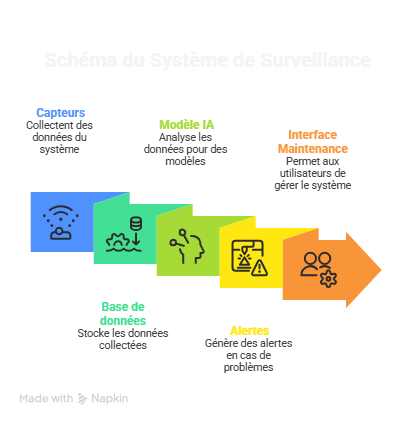
\includegraphics[width=0.85\textwidth]{Intégration d'un Module d'Intelligence Artificielle dans un Système de Surveillance - visual selection (2).png}
\caption{Position du module IA dans le système global}
\end{figure}

\section{Collecte et préparation des données}

\subsection{Source des données}

Les données sont stockées dans MongoDB, dans la collection \texttt{sensordatas}. Cette collection contient les mesures envoyées par les capteurs installés sur les machines.

\subsection{Variables utilisées}

Les variables d’entrée utilisées par le modèle sont :
\begin{itemize}
\item \texttt{vibX}, \texttt{vibY}, \texttt{vibZ} : vibrations selon les trois axes
\item \texttt{courant} : courant électrique consommé
\item \texttt{rpm} : vitesse de rotation
\item \texttt{pression} : pression mesurée
\end{itemize}

Ces variables représentent les \textbf{features}. La sortie attendue correspond à l’état de la machine.

\subsection{Construction du dataset}

Les données ont été extraites depuis MongoDB puis transformées en fichier CSV nommé \texttt{Lstm\_dataset.csv}. Ce fichier est utilisé comme base d’apprentissage.

\begin{figure}[H]
\centering
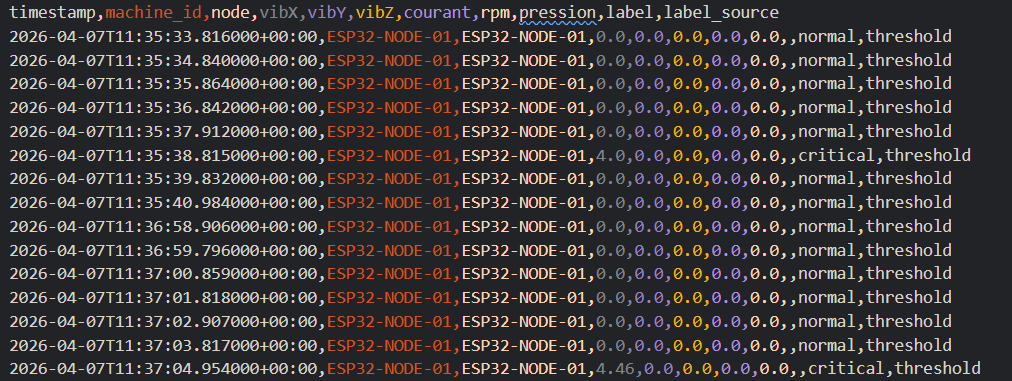
\includegraphics[width=0.85\textwidth]{Capture d’écran 2026-04-26 000837.png}
\caption{Exemple du dataset utilisé pour l’apprentissage}
\end{figure}

\subsection{Étiquetage des données}

Les données sont classées en trois catégories :
\begin{itemize}
\item \textbf{Normal} : fonctionnement stable
\item \textbf{Warning} : comportement anormal nécessitant une surveillance
\item \textbf{Critical} : état critique indiquant un risque de panne
\end{itemize}

Une partie des labels est générée à partir de seuils métiers afin de créer un dataset initial pour l’entraînement.

\subsection{Pré-traitement des données}

Avant l’entraînement, les données passent par une phase de pré-traitement :
\begin{itemize}
\item Nettoyage des données
\item Gestion des valeurs manquantes
\item Suppression des valeurs aberrantes
\item Normalisation des valeurs numériques
\end{itemize}

La normalisation est importante pour éviter qu’une variable domine les autres pendant l’apprentissage.

\section{Choix et entraînement du modèle IA}

\subsection{Nature du problème}

Le problème traité est un problème de \textbf{Machine Learning supervisé} de type \textbf{classification multi-classes}.

Le modèle apprend à partir de données étiquetées afin de reconnaître les états possibles de la machine.

\subsection{Modèle choisi}

Le modèle utilisé est un réseau de neurones de type \textbf{LSTM} (\textit{Long Short-Term Memory}).

Ce choix est adapté car les données capteurs sont des \textbf{séries temporelles}. Le LSTM peut analyser l’évolution des mesures dans le temps et détecter des anomalies progressives.

\subsection{Principe}

Contrairement à une analyse basée sur une seule mesure isolée, le modèle LSTM analyse une séquence de mesures successives. Cela permet d’identifier les changements de comportement de la machine.

\begin{figure}[H]
\centering
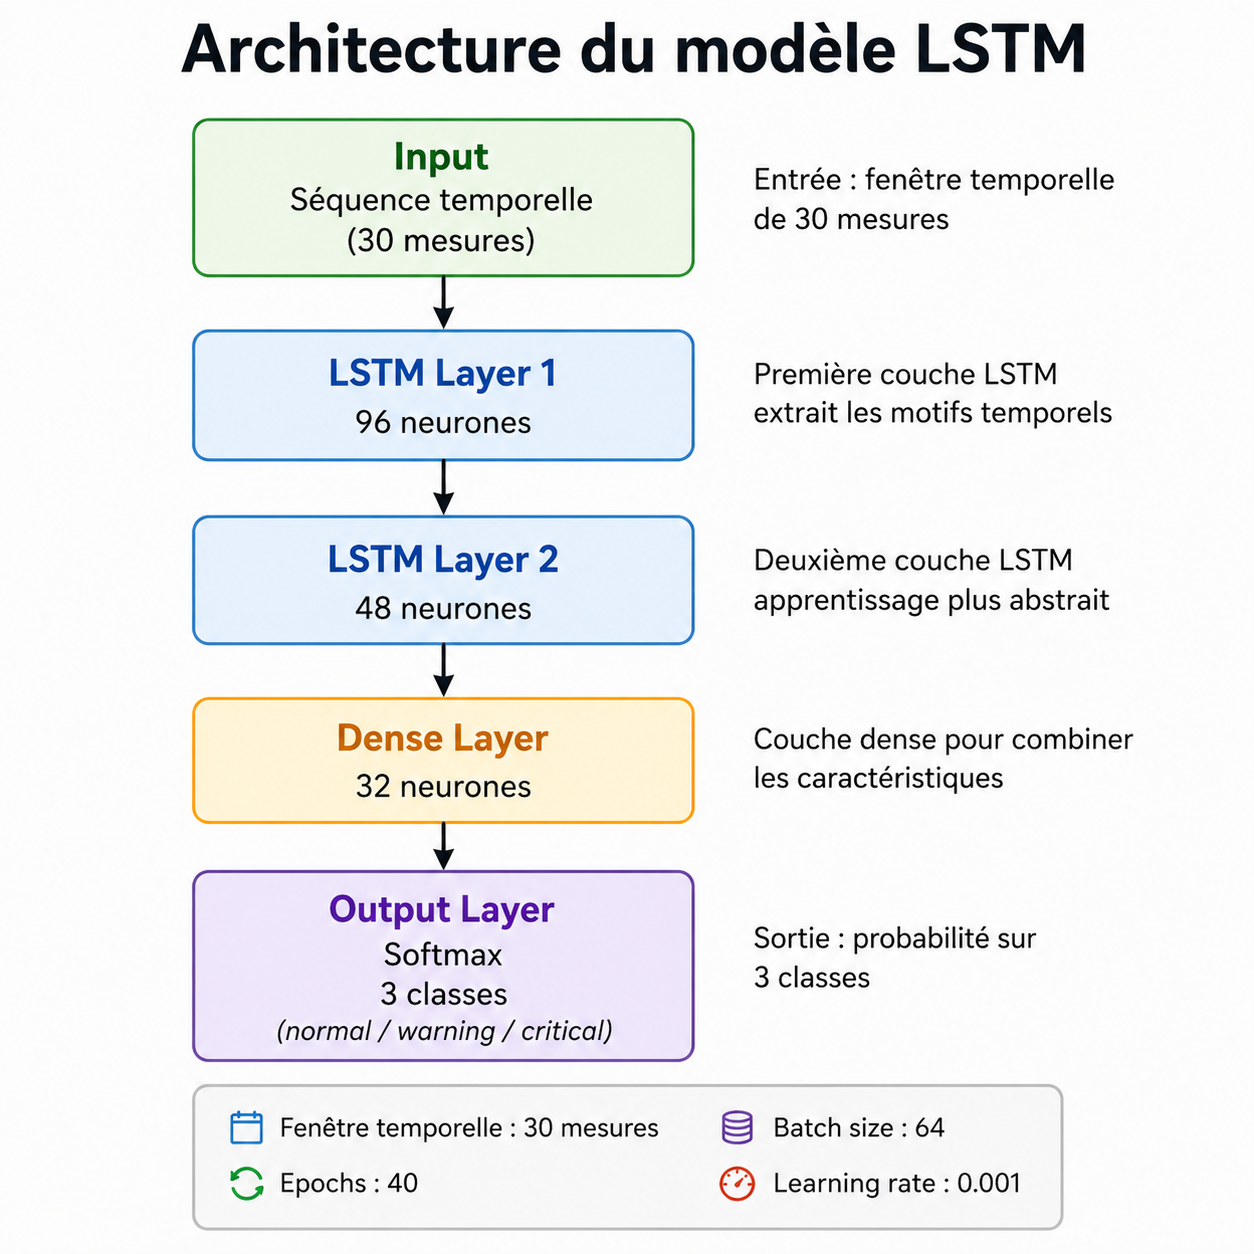
\includegraphics[width=0.8\textwidth]{ChatGPT Image Apr 26, 2026, 12_46_24 AM.png}
\caption{Architecture du modèle LSTM}
\end{figure}

\subsection{Entraînement du modèle}

L’entraînement du modèle a été réalisé sur 40 epochs. À chaque epoch, le modèle ajuste ses poids afin de réduire l’erreur entre la prédiction et la valeur réelle.

L’apprentissage est suivi à travers :
\begin{itemize}
\item L’accuracy
\item La loss
\end{itemize}

\begin{figure}[H]
\centering
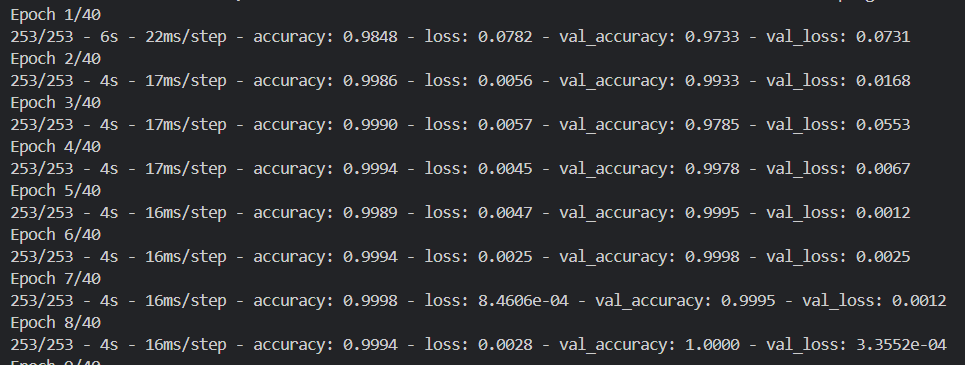
\includegraphics[width=0.9\textwidth]{train.png}
\caption{Exemple des logs d’entraînement du modèle LSTM}
\end{figure}

\subsection{Gestion du déséquilibre des classes}

Le dataset contient un déséquilibre entre les classes, notamment pour la classe \textit{warning}. Pour limiter ce problème, une génération synthétique a été utilisée afin d’augmenter les classes rares.

\section{Résultats et évaluation}

\subsection{Données utilisées}

Le dataset contient 12 818 lignes collectées à partir de deux machines industrielles.

\subsection{Évolution de l’entraînement}

Les courbes de loss et d’accuracy permettent de suivre l’évolution du modèle pendant l’apprentissage.

\begin{figure}[H]
\centering
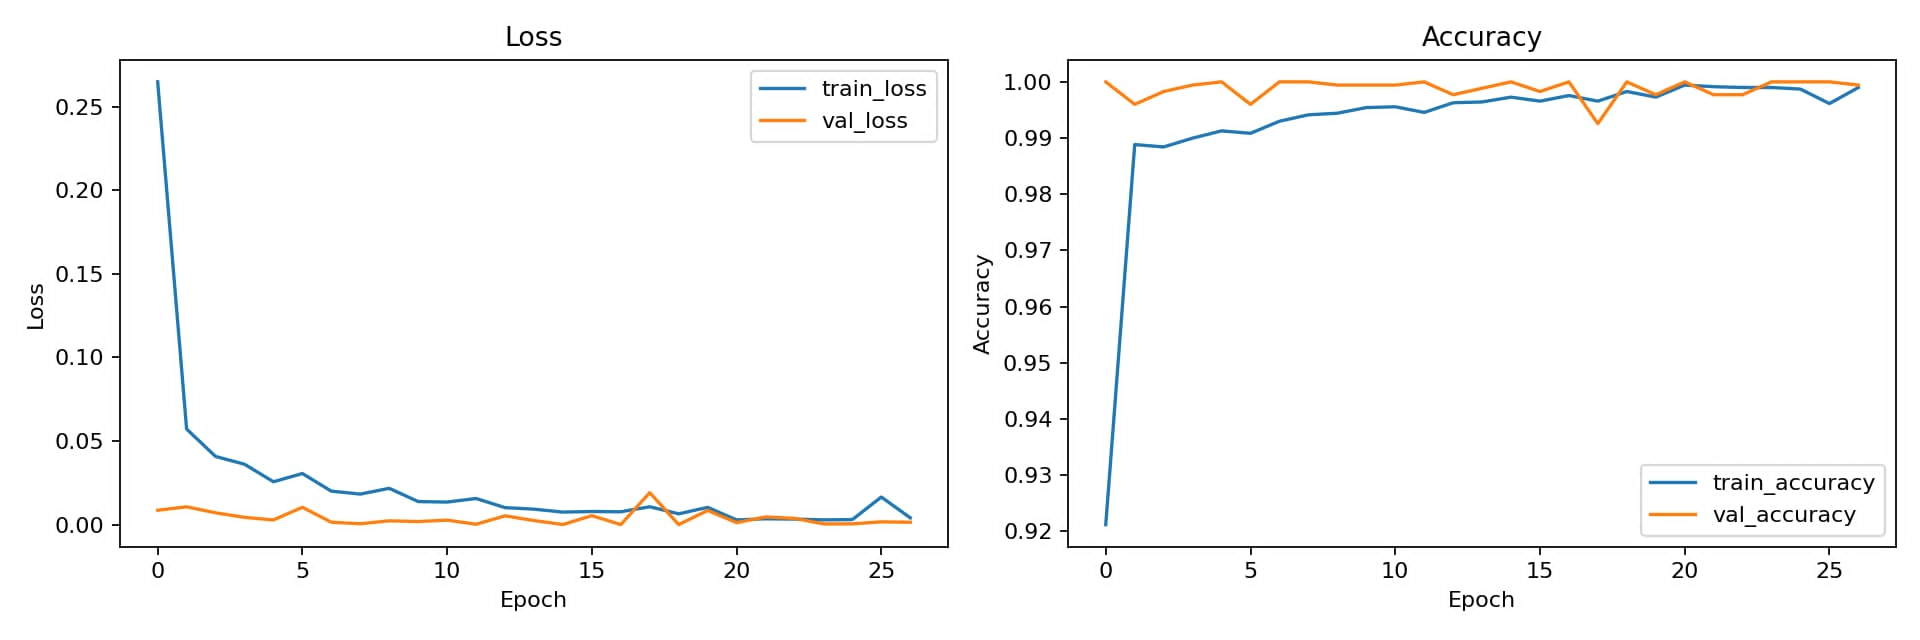
\includegraphics[width=0.95\textwidth]{7abef080-e8a1-4790-8853-731e269001b4.jpg}
\caption{Évolution de la loss et de l’accuracy pendant l’entraînement}
\end{figure}

\subsection{Matrice de confusion}

La matrice de confusion permet d’analyser les prédictions correctes et incorrectes pour chaque classe.

\begin{figure}[H]
\centering
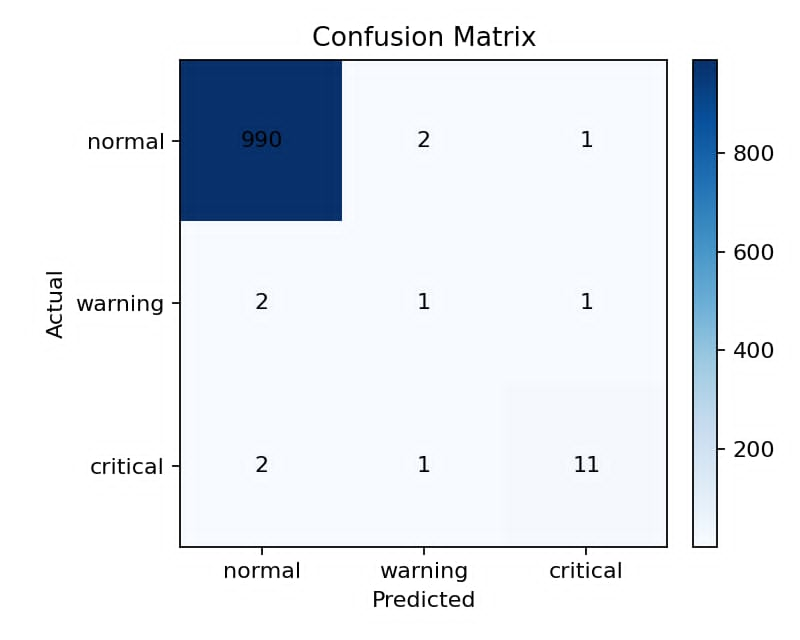
\includegraphics[width=0.75\textwidth]{03082855-de7c-46e7-ad10-46fe5cd5954d.jpg}
\caption{Matrice de confusion du modèle LSTM}
\end{figure}

\subsection{Résultat}

Le modèle donne de bons résultats, surtout pour les états \textit{normal} et \textit{critical}. La classe \textit{warning} reste plus difficile à prédire à cause du nombre limité d’exemples.

\subsection{Score d’anomalie}

Dans l’application, la sortie principale n’est pas seulement une classe comme \textit{normal}, \textit{warning} ou \textit{critical}. Le modèle fournit aussi un \textbf{score d’anomalie} exprimé en pourcentage.

Ce score représente le niveau de risque détecté par l’IA :
\begin{itemize}
\item 0\% -- 40\% : fonctionnement normal
\item 40\% -- 70\% : état de surveillance
\item 70\% -- 100\% : risque critique
\end{itemize}

Cette approche permet une décision plus progressive. Au lieu d’afficher uniquement une classe, le système indique le niveau de danger réel.

\section{Intégration dans l’application}

Le module IA est intégré dans l’application afin d’analyser les données capteurs en temps réel via MQTT.

\subsection{Fonctionnalités du système}

\begin{table}[H]
\centering
\begin{tabular}{|l|p{10cm}|}
\hline
\textbf{Fonctionnalité} & \textbf{Description} \\
\hline
Inférence temps réel & Analyse continue des données capteurs via MQTT \\
\hline
Score d’anomalie & Affichage du niveau de risque en pourcentage \\
\hline
Alertes automatiques & Détection des anomalies et génération d’alertes \\
\hline
Diagnostic IA & Interprétation du résultat, par exemple panne probable \\
\hline
Demandes maintenance & Création et suivi des interventions \\
\hline
\end{tabular}
\caption{Fonctionnalités du module IA dans l’application}
\end{table}

\subsection{Interface utilisateur}

L’interface permet de visualiser en temps réel les résultats du modèle IA ainsi que les informations de maintenance.

\begin{figure}[H]
\centering
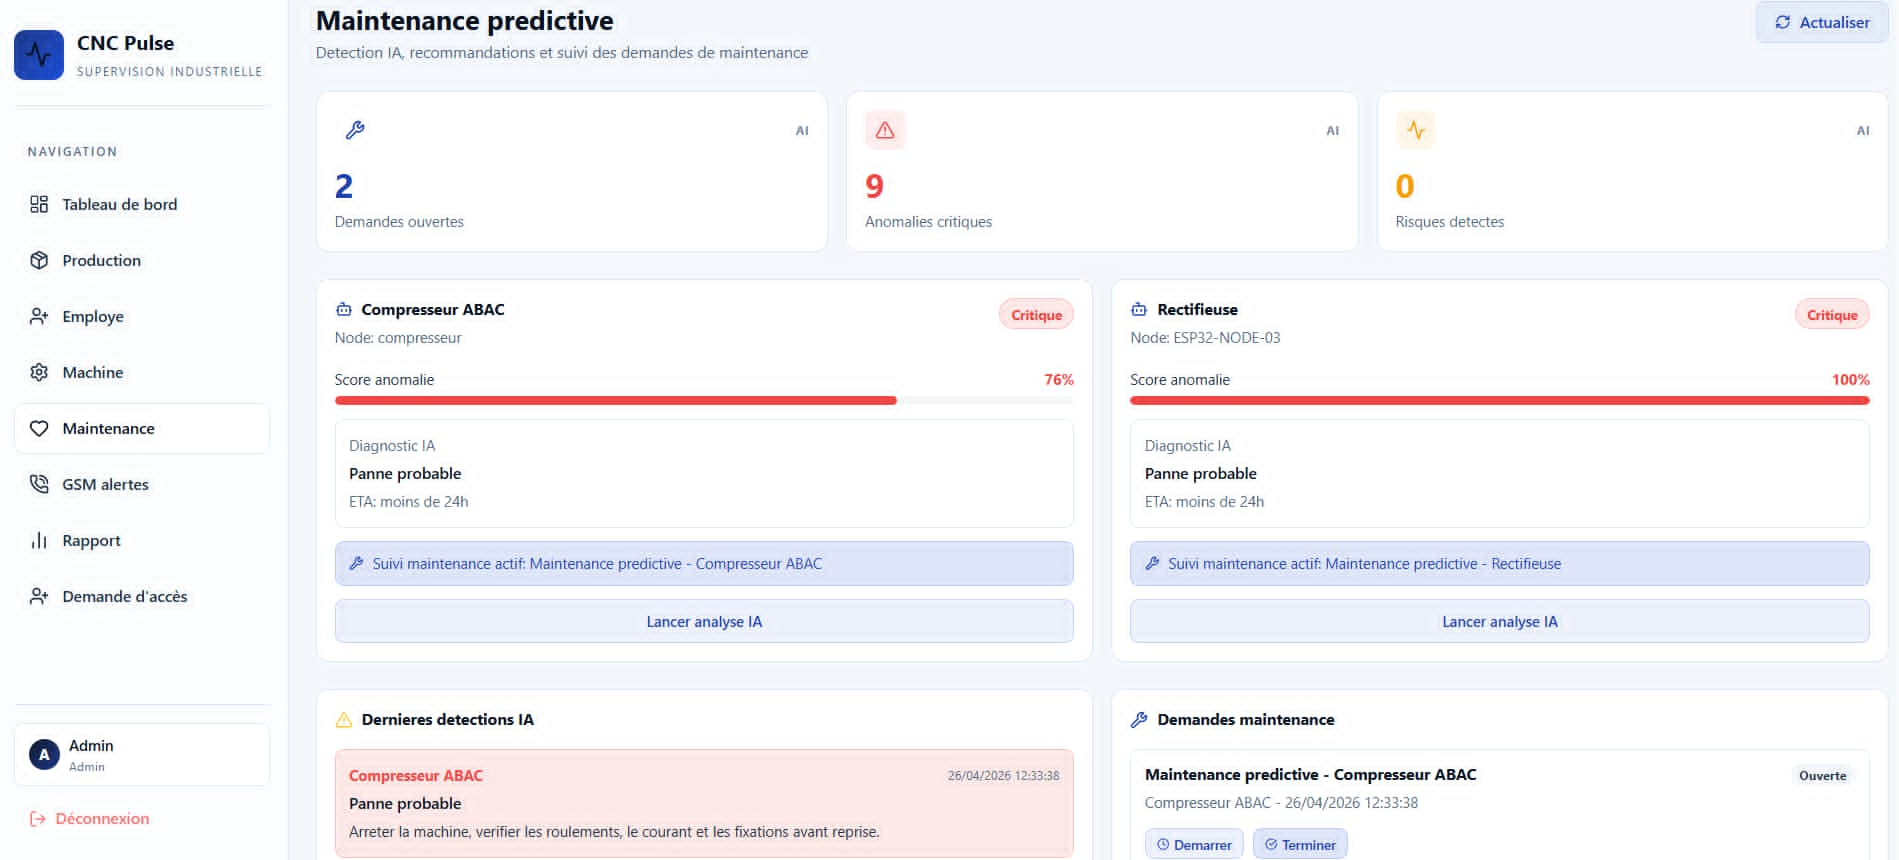
\includegraphics[width=0.95\textwidth]{73eea2cd-a194-4b31-832e-9f57ce25a37d.jpg}
\caption{Interface de maintenance prédictive et supervision des machines}
\end{figure}

\subsection{Fonctionnalités visibles dans l’interface}

\begin{table}[H]
\centering
\begin{tabular}{|l|p{10cm}|}
\hline
\textbf{Élément} & \textbf{Description} \\
\hline
Score anomalie & Indique le niveau de risque détecté par l’IA \\
\hline
État machine & Affiche l’interprétation générale de l’état \\
\hline
Diagnostic IA & Donne une explication comme panne probable \\
\hline
ETA & Temps estimé avant panne \\
\hline
Alertes & Notifications automatiques en cas d’anomalie \\
\hline
Demandes maintenance & Suivi des interventions ouvertes \\
\hline
\end{tabular}
\caption{Fonctionnalités affichées dans l’interface}
\end{table}

\section{Analyse critique}

Malgré les bons résultats, certaines limites restent présentes :
\begin{itemize}
\item Dataset limité à deux machines
\item Déséquilibre entre les classes
\item Classe warning difficile à prédire
\item Labels initiaux basés sur des seuils métiers
\end{itemize}

\section{Conclusion et perspectives}

Dans ce projet, nous avons développé un module d’intelligence artificielle dédié à la maintenance prédictive des machines industrielles, basé sur l’analyse des données issues des capteurs.

Le choix du modèle LSTM s’est avéré pertinent, car il permet de traiter les données temporelles et de détecter les anomalies de manière progressive. Contrairement aux approches classiques, le modèle apprend automatiquement les comportements de la machine à partir des données.

L’un des points importants de ce travail est l’utilisation d’un score d’anomalie. Ce score permet d’avoir une vision plus précise du niveau de risque, au lieu de se limiter à une simple classification. Il facilite ainsi la prise de décision en maintenance.

Les résultats obtenus sont satisfaisants, notamment pour les états normal et critical. Toutefois, certaines limites existent, comme le déséquilibre des classes et le nombre limité de données.

Pour améliorer le système, il serait intéressant d’ajouter plus de données réelles et de tester d’autres modèles afin d’augmenter la précision et la robustesse du modèle.

Ce projet montre l’intérêt de l’intelligence artificielle pour améliorer la maintenance industrielle en rendant les systèmes plus prédictifs et efficaces.

\end{document}